%==============================================================================
% Exact and Structural Methods for the Job Sequencing and Tool Switching Problem
% Mid-internship report.
%
% Build:  pdflatex mid_internship_report && bibtex mid_internship_report &&
%         pdflatex mid_internship_report && pdflatex mid_internship_report
%
% Authoring/expansion notes are kept OUT of this file (see AI_EXPANSION_GUIDE.md)
% so that the document itself is standalone.
%==============================================================================
\documentclass[11pt,a4paper]{article}

\usepackage{lmodern}
\usepackage[T1]{fontenc}
\usepackage[utf8]{inputenc}
\usepackage[margin=1in]{geometry}
\usepackage{amsmath,amssymb,amsthm,mathtools}
\usepackage{booktabs}
\usepackage{enumitem}
\usepackage{tikz}
\usepackage[numbers,sort&compress]{natbib}
\usepackage[hidelinks]{hyperref}

\theoremstyle{plain}
\newtheorem{theorem}{Theorem}
\newtheorem{lemma}{Lemma}
\newtheorem{proposition}{Proposition}
\newtheorem{corollary}{Corollary}
\theoremstyle{definition}
\newtheorem{definition}{Definition}
\newtheorem{conjecture}{Conjecture}
\newtheorem{problem}{Problem}
\theoremstyle{remark}
\newtheorem{remark}{Remark}
\newtheorem{example}{Example}

\DeclareMathOperator{\KTNS}{KTNS}
\newcommand{\U}{U}
\newcommand{\Kst}{K^{\ast}}
\newcommand{\Zst}{Z^{\ast}}
\newcommand{\confs}{\mathcal{C}}
\newcommand{\rset}[1]{\{#1\}}

\title{\textbf{Exact and Structural Methods for the\\
Job Sequencing and Tool Switching Problem}\\[4pt]
\large Mid-internship report}
\author{%
  Shankar Narayanan\thanks{\texttt{shajaganbpgc@gmail.com}}\\[6pt]
  \normalsize Project advisors: Dr.\ Rafael Colares \quad Prof.\ Annegret Wagler\\
  \normalsize Academic supervisor: Dr.\ Renaud Chicoisne%
  % TODO: add laboratory (e.g.\ LIMOS, Universit\'e Clermont Auvergne) and internship dates.
}
\date{\today}

\begin{document}
\maketitle

\begin{abstract}
The Job Sequencing and Tool Switching Problem (SSP) asks for an ordering of a set
of jobs on a single flexible machine, together with a tool-loading policy for a
capacitated tool magazine, that minimises the number of tool switches. This report
develops \emph{exact} and \emph{structural} methods for the SSP. Two pillars
organise the work, joined by a single geometric lens---the equivalence between the
SSP and a generalised travelling-salesman problem over tool \emph{configurations}.
The first pillar is a structural analysis of the natural two-phase heuristic (group
the jobs, then order the groups): we prove that the SSP optimum equals the minimum
generalised-TSP cost over \emph{all} feasible groupings, which shows the
heuristic's optimality gap to be exactly the price of insisting on a
minimum-cardinality grouping; we then give matching lower bounds, a family on which
the gap grows without bound, an unconditional approximation-ratio bound, and two
conjectures supported by exhaustive computation. The second pillar is exact
computation: a branch-and-Benders-cut algorithm whose subproblem is the polynomial
tool-loading oracle, and a family of position-indexed formulations with a fixed,
polynomial row set together with an exact branch-and-price. We close with an
objective assessment of why a configuration-based branch-and-price for the SSP is
\emph{bound-limited} rather than implementation-limited. Results established here
are stated as theorems and propositions; results supported by exhaustive
enumeration but not yet proved are stated as conjectures, with the scope of the
supporting experiments made explicit. Longer proofs are collected in the appendix.
\end{abstract}

\tableofcontents

%==============================================================================
\section{Introduction}\label{sec:intro}
%==============================================================================
\paragraph{Motivation.}
A flexible manufacturing cell built around a single computer-numerically-controlled
machine can produce a wide variety of parts because it draws on a large library of
cutting tools. The machine, however, holds only a limited number of tools at once,
in a magazine of capacity~$b$; producing the full part mix therefore requires tools
to be exchanged between jobs. Each exchange interrupts production while the magazine
is reconfigured, so tool switches are the dominant controllable cost in such cells
\citep{Crama1994}. When the set of tools needed by each job is fixed, two decisions
remain: in what \emph{order} to process the jobs, and which tools to \emph{keep or
evict} at each step. The Job Sequencing and Tool Switching Problem (SSP) is the
joint optimisation of these two decisions so as to minimise the total number of
switches. The same structure---a capacitated store serving set-valued requests that
may be reordered---recurs beyond machining, for example in printed-circuit-board
assembly and in warehouse order picking, so the methods developed here are not
specific to tools.

\paragraph{Why the problem is subtle.}
The two decisions are coupled in opposite directions. For a \emph{fixed} job order,
the optimal loading policy is known in closed form---the Keep Tool Needed Soonest
(KTNS) rule of \citet{Tang1988}, computable in $O(n\lvert T\rvert)$ time---so the
loading subproblem is easy. The difficulty lies entirely in the ordering: a good
order places jobs with similar tool requirements next to one another so that few
tools change hands, but ``similarity'' here is a set-overlap relation with no
underlying metric, and the capacity constraint couples positions that are far apart
in the sequence. The joint problem is NP-hard \citep{Crama1994,Laporte2004}, and
even the strongest compact integer formulations \citep{Catanzaro2015,Laporte2004,%
daSilva2024} become difficult beyond moderate sizes. This structure---an easy inner
problem nested inside a hard ordering problem---is precisely what decomposition
methods are designed to exploit, and it motivates both pillars of this work.

\paragraph{Two pillars and a common lens.}
The report is organised around two complementary questions.
\begin{enumerate}[noitemsep,topsep=2pt]
  \item \textbf{How good is the natural heuristic?} A widely used two-phase method
  first partitions the jobs into the fewest groups whose tool requirements each fit
  in the magazine (the Job Grouping Problem, JGP), then orders the groups by solving
  a travelling-salesman-type problem, and finally reads off a schedule. We ask how
  far this heuristic can be from optimal, and when it is exact.
  \item \textbf{How does one solve the SSP exactly, and how fast?} We develop a
  branch-and-Benders-cut algorithm and a family of position-indexed formulations
  with an exact branch-and-price, and assess their competitiveness.
\end{enumerate}
Both pillars are most naturally expressed in one geometry. A \emph{tool
configuration} is a magazine-filling set of tools; the SSP is then a generalised
travelling-salesman problem (GTSP) that must visit, in some order, one configuration
able to serve each job, paying for the tools that change between consecutive
configurations \citep{Colares2026Exact}. This configuration--GTSP equivalence
(Section~\ref{sec:prelim}) is the thread tying the heuristic analysis to the exact
formulations, and we establish it once, at the outset.

\paragraph{Contributions.}
The principal results are the following.
\begin{itemize}[noitemsep,topsep=2pt]
  \item \emph{A reframing of the heuristic gap} (Section~\ref{sec:gap}): we prove
  that the SSP optimum equals the minimum GTSP cost over \emph{all} feasible
  groupings, not only minimum-cardinality ones. Consequently the two-phase
  heuristic's optimality gap is exactly the cost of restricting attention to
  minimum-cardinality groupings.
  \item \emph{Gap quantification}: we prove the matching lower bounds $\Zst\ge
  \max(\Kst-1,\lvert\U\rvert-b)$ and that the two-phase heuristic is a
  $b$-approximation; we exhibit a family on which the gap grows linearly without
  bound; and we state two conjectures---$H/\Zst\le 4/3$ for $b=3$, and
  $\mathrm{gap}\le\Kst-2$---each unfalsified by exhaustive enumeration over many
  thousands of instances.
  \item \emph{A collapse theorem}: under a per-changeover magazine setup cost, the
  heuristic becomes exact once the ratio of setup cost to switch cost exceeds an
  explicit threshold.
  \item \emph{Exact methods} (Section~\ref{sec:exact}): a branch-and-Benders-cut
  solver whose subproblem is the polynomial KTNS oracle, verified optimal against
  exhaustive search; and position-indexed formulations (PCF, its symmetry-reduced
  variant PCF$'$, and the transition model PTF) with a fixed $O(n\lvert T\rvert)$ row
  set, their pricing subproblems, and an exact branch-and-price.
  \item \emph{An objective competitiveness assessment} (Section~\ref{sec:comp}):
  for the SSP the configuration relaxation collapses to the trivial coverage bound
  on most instances, so a configuration-based branch-and-price is bound-limited
  rather than implementation-limited.
\end{itemize}

\paragraph{Outline.}
Section~\ref{sec:prelim} fixes notation, defines the SSP and KTNS, introduces the
two-phase heuristic and the configuration--GTSP lens, proves the two structural
lower bounds, fixes the switch-cost convention, and reviews the literature.
Section~\ref{sec:gap} develops the structural theory of the heuristic gap;
Section~\ref{sec:exact} presents the exact methods; Section~\ref{sec:comp} reports
the experimental design, the verification of correctness, and the competitiveness
assessment; and Section~\ref{sec:concl} concludes with open problems and future
directions. Longer proofs are deferred to Appendix~\ref{app:proofs}.

%==============================================================================
\section{Preliminaries}\label{sec:prelim}
%==============================================================================

\subsection{The Job Sequencing and Tool Switching Problem}\label{ssec:ssp}
We are given $n$ jobs $J=\rset{1,\dots,n}$, $m$ tools $T=\rset{1,\dots,m}$, a
magazine capacity $b\in\mathbb{N}$ with $b<m$, and for each job $j$ a set of
required tools $T_j\subseteq T$ with $1\le\lvert T_j\rvert\le b$. We write
$\U=\bigcup_{j\in J}T_j$ for the set of tools used by at least one job.

\begin{definition}[Schedule and switch cost]\label{def:ssp}
A \emph{schedule} is a pair $(\pi,\mathbf{M})$ consisting of a permutation $\pi$ of
$J$ and a sequence of \emph{magazine states} $\mathbf{M}=(M_1,\dots,M_n)$, $M_i
\subseteq T$, satisfying the capacity and feasibility constraints
\[
  \lvert M_i\rvert\le b \quad\text{and}\quad T_{\pi(i)}\subseteq M_i
  \qquad (i=1,\dots,n).
\]
With $M_0=\varnothing$, its \emph{switch cost} is the total number of tool
insertions, $\sum_{i=1}^{n}\lvert M_i\setminus M_{i-1}\rvert$. The SSP asks for a
schedule of minimum switch cost; this optimum is denoted~$\Zst$.
\end{definition}

Counting insertions is the standard cost model: under a fixed capacity each
insertion into a full magazine forces exactly one removal, so insertions and
removals differ only by boundary terms, which Section~\ref{ssec:conv} makes precise.

\begin{example}[A running instance: the $6$-ring]\label{ex:ring}
We illustrate every definition on one instance, returned to throughout
(Figure~\ref{fig:ring}). The \emph{$6$-ring} has $n=m=6$, capacity $b=3$, and
$T_j=\{j,j+1\}$ with indices taken
modulo $6$ (so $T_6=\{6,1\}$); the jobs form a cycle in which consecutive jobs share
exactly one tool. Its job--tool incidence matrix (rows are tools $1$--$6$, columns
jobs $1$--$6$; a blank denotes $0$) is
\[
\begin{array}{c|cccccc}
      & 1 & 2 & 3 & 4 & 5 & 6\\\hline
 t_1  & 1 &   &   &   &   & 1\\
 t_2  & 1 & 1 &   &   &   &  \\
 t_3  &   & 1 & 1 &   &   &  \\
 t_4  &   &   & 1 & 1 &   &  \\
 t_5  &   &   &   & 1 & 1 &  \\
 t_6  &   &   &   &   & 1 & 1
\end{array}
\]
Process the jobs in the cyclic order $1,2,3,4,5,6$ and load by the rule of
Section~\ref{ssec:ktns}. The magazine evolves as
\[
\{1,2,3\}\;\to\;\{1,2,3\}\;\to\;\{1,3,4\}\;\to\;\{1,4,5\}\;\to\;\{1,5,6\}\;\to\;
\{1,5,6\},
\]
inserting $3$ tools to build the first magazine and then one tool at each of
positions $3,4,5$: a switch cost of $6$, equivalently $3$ once the initial fill is
not charged (Section~\ref{ssec:conv}). Section~\ref{sec:gap} shows that $6$ is
optimal, yet the two-phase heuristic of Section~\ref{ssec:jgp} returns $7$. The
$6$-ring is thus the smallest instance on which grouping-then-sequencing is provably
sub-optimal, and it recurs below as the canonical witness of a positive gap.
\end{example}

\begin{figure}[h]\centering
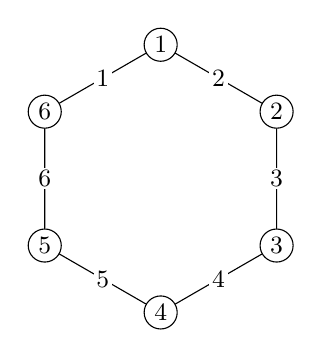
\begin{tikzpicture}[scale=1.7,line cap=round,every node/.style={font=\small}]
  \foreach \i in {1,...,6}{
    \node[draw,circle,fill=white,inner sep=1.6pt] (j\i) at ({90-(\i-1)*60}:1) {$\i$};
  }
  \foreach \a/\b/\t in {1/2/2,2/3/3,3/4/4,4/5/5,5/6/6,6/1/1}{
    \draw (j\a)--(j\b) node[midway,fill=white,inner sep=1pt]{$\t$};
  }
\end{tikzpicture}
\caption{The $6$-ring. Jobs $1$--$6$ lie on a cycle; each edge is labelled by the
single tool its two endpoints share ($T_j=\{j,j+1\}$). Adjacent jobs overlap in one
tool; non-adjacent jobs are tool-disjoint.}\label{fig:ring}
\end{figure}

\subsection{The tool-loading oracle}\label{ssec:ktns}
The inner problem---optimal loading for a fixed order---is solved by a greedy rule
whose optimality is classical.
\begin{proposition}[\citealp{Tang1988}]\label{prop:ktns}
For a fixed permutation $\pi$, an optimal magazine sequence is produced by the
\emph{Keep Tool Needed Soonest} (KTNS) policy: whenever a tool must be inserted into
a full magazine, evict a tool whose next required use lies furthest in the future
(evicting any tool never required again). KTNS runs in $O(n\lvert T\rvert)$ time and
returns the minimum switch cost over all loading policies for~$\pi$.
\end{proposition}
A proof appears in \citet{Tang1988}; see also \citet{Crama1994}. KTNS reduces the
SSP to a pure sequencing problem, $\Zst=\min_{\pi}\KTNS(\pi)$, and is the exact
polynomial subproblem exploited by the Benders algorithm of
Section~\ref{ssec:bbc}.

\begin{remark}[The loading subproblem is offline optimal caching]\label{rem:belady}
For a fixed order the loading problem is exactly offline paging: the magazine is a
cache of size $b$, position $i$ requests the set $T_{\pi(i)}$, and an insertion is a
cache miss. Proposition~\ref{prop:ktns} is then the tool-switching form of
B\'el\'ady's optimal replacement rule---evict the item whose next request is
furthest in the future---which minimises misses on any fixed request sequence
\citep{Belady1966}. The contrast with the full problem is instructive: paging fixes
the request order, whereas the SSP may \emph{reorder} the jobs, and it is precisely
this freedom that turns a polynomially solvable caching problem into an NP-hard one.
Every method in this report is, at heart, a way to search over reorderings while
delegating the loading to this exact oracle.
\end{remark}

\subsection{Grouping, sequencing, and the two-phase heuristic}\label{ssec:jgp}
A complementary viewpoint ignores order and asks only which jobs may \emph{share} a
magazine.
\begin{definition}[Job Grouping Problem]\label{def:jgp}
A \emph{group} is a set of jobs $G\subseteq J$ whose combined tool requirement fits
in the magazine, $\lvert\bigcup_{j\in G}T_j\rvert\le b$. The Job Grouping Problem
(JGP) partitions $J$ into the minimum number $\Kst$ of groups; equivalently, it
covers all jobs by the fewest tool configurations of size at most~$b$.
\end{definition}
The JGP is itself NP-hard and is solved exactly by the asymmetric-representatives
formulation of \citet{Jans2013} or by the set-covering column generation of
\citet{Crama1994Column}. It induces the classical two-phase heuristic for the SSP:
\begin{enumerate}[noitemsep,topsep=2pt]
  \item solve the JGP to obtain $\Kst$ groups and a configuration serving each;
  \item solve the \emph{Group Sequencing Problem}---order the configurations by a
  travelling-salesman-type problem whose transition cost is the number of tools that
  change, a small instance handled by standard solvers
  \citep{Applegate2006,Helsgaun2015}---to obtain a sequence of configurations;
  \item concatenate the jobs group by group and evaluate the resulting order with
  KTNS.
\end{enumerate}
We write $H$ for the switch cost this heuristic returns. Since it produces a
feasible schedule, $H\ge\Zst$ always; the objects of study are the \emph{gap}
$H-\Zst$ and the \emph{ratio} $H/\Zst$ (Section~\ref{sec:gap}).

\begin{example}[Grouping the $6$-ring]\label{ex:ring-group}
On the running instance the JGP returns $\Kst=3$; one optimal grouping is
$\{1,2\},\{3,4\},\{5,6\}$, served by the configurations $\{1,2,3\}$, $\{3,4,5\}$,
$\{5,6,1\}$. Any two of these three configurations differ in two tools, so every
ordering of the groups changes two tools at each of its two transitions, and the
best schedule the heuristic produces costs $H=7$ (free-initial~$4$). This is one
more than the optimum of $6$ (free-initial~$3$) attained in Example~\ref{ex:ring}:
a gap of exactly one. The discrepancy is not a failure of the sequencing phase---the
groups are ordered optimally---but of the \emph{grouping} phase, which insists on
only $\Kst=3$ groups; Section~\ref{sec:gap} makes this precise.
\end{example}

\subsection{The configuration--GTSP lens}\label{ssec:gtsp}
Both the heuristic and the exact formulations live in the space of configurations.
\begin{definition}[Configurations and clusters]\label{def:config}
A \emph{configuration} is a set $C\subseteq T$ with $\lvert C\rvert=b$. Let
$\confs=\rset{C\subseteq T:\lvert C\rvert=b}$, and for each job $j$ let $H_j=
\rset{C\in\confs:T_j\subseteq C}$ be the \emph{cluster} of configurations able to
serve~$j$. For configurations $C,C'$ put $d(C,C')=\lvert C'\setminus C\rvert$, the
number of tools inserted in passing from $C$ to~$C'$.
\end{definition}
Restricting to full magazines ($\lvert C\rvert=b$) loses no optimality: retaining a
tool that may be useful later never increases cost. Under this view a schedule is a
walk $C_{(1)},\dots,C_{(r)}$ in $\confs$ that visits at least one configuration of
every cluster $H_j$, with cost $\sum_l d(C_{(l)},C_{(l+1)})$; the SSP is therefore a
\emph{generalised travelling-salesman problem with overlapping clusters} over
$\confs$ \citep{Colares2026Exact}. The clusters $H_j$ overlap---a rich configuration
serves many jobs---which is exactly what distinguishes the SSP from a textbook GTSP
with disjoint clusters \citep{Noon1993,Fischetti1997,Pop2024}. That a schedule and such a covering walk have equal cost is immediate in one
direction---the distinct consecutive magazines of any schedule form a covering walk
of the same cost---and the converse is established, in the stronger form ranging
over \emph{all} feasible groupings, as Theorem~\ref{thm:grouping} of
Section~\ref{sec:gap} (proof in Appendix~\ref{app:proofs}). This lens recurs
throughout: it underlies the gap analysis of Section~\ref{sec:gap}, the
position-indexed formulations of Section~\ref{ssec:pos}, and the reading of the
Benders master as a travelling-salesman skeleton (Section~\ref{ssec:bbc}).

\subsection{Two structural lower bounds}\label{ssec:lb}
The following bounds are elementary but pervasive: they drive the gap theory of
Section~\ref{sec:gap}, calibrate the linear relaxations of
Section~\ref{sec:exact}, and serve as correctness checks for the computational
study. Both are stated in the \emph{free-initial} cost (Section~\ref{ssec:conv}),
which does not charge the first magazine fill; the conversion to
Definition~\ref{def:ssp} is the additive constant of Proposition~\ref{prop:conv}.

\begin{proposition}[Grouping bound]\label{prop:lb1}
$\Zst\ge\Kst-1$.
\end{proposition}
\begin{proof}
Fix any schedule and list its magazine states $M_1,\dots,M_n$; collapse each
maximal run of equal states to a single representative, obtaining a sequence
$C_{(1)},\dots,C_{(r)}$ in which consecutive entries differ. Every job is served by
some state, hence by some $C_{(l)}$, so $\rset{C_{(1)},\dots,C_{(r)}}$ is a family of
sets of size at most $b$ covering all jobs. Assigning each job to one configuration
that contains its requirement partitions $J$ into groups, one per \emph{distinct}
configuration, each group having combined requirement contained in that
configuration and hence of size at most~$b$; this is a feasible grouping, so the
number of distinct configurations is at least~$\Kst$. Therefore $r\ge\Kst$. Finally,
each of the $r-1$ consecutive transitions changes at least one tool, so the
free-initial switch cost is at least $r-1\ge\Kst-1$.
\end{proof}

\begin{proposition}[Coverage bound]\label{prop:lb2}
$\Zst\ge\lvert\U\rvert-b$.
\end{proposition}
\begin{proof}
Each tool of $\U$ is required by some job and therefore occupies the magazine at
some position, so it is inserted at least once unless it belongs to the initial fill,
which contains at most $b$ tools. Hence at least $\lvert\U\rvert-b$ insertions occur
in the free-initial count.
\end{proof}

\begin{corollary}\label{cor:lb}
$\Zst\ge\max\rset{\Kst-1,\ \lvert\U\rvert-b}$.
\end{corollary}

\noindent The two bounds are individually tight on some families and simultaneously
slack on others (Section~\ref{sec:gap}). The coverage bound $\lvert\U\rvert-b$ is
exactly the value to which the multicommodity-flow relaxation of \citet{daSilva2024}
collapses---a fact central to the assessment of Section~\ref{ssec:assess}. The two
are genuinely different measurements: on the $6$-ring, $\Kst-1=2$ while
$\lvert\U\rvert-b=6-3=3$, so the coverage bound is tight ($\Zst=3$ free-initial,
Example~\ref{ex:ring}) and the grouping bound is slack, whereas on instances built
from many nearly tool-disjoint groups the reverse holds. Neither dominates in
general, and Section~\ref{sec:gap} shows that their maximum, though always valid, is
not always attained.

\subsection{Switch-cost convention}\label{ssec:conv}
Formulations in the literature charge the initial magazine fill differently, and
comparing their objective values naively produces spurious discrepancies; we
therefore fix the convention.
\begin{definition}[Empty-start and free-initial costs]\label{def:conv}
The \emph{empty-start} cost charges every insertion from an initially empty magazine
($M_0=\varnothing$, as in Definition~\ref{def:ssp}). The \emph{free-initial} cost
does not charge the first fill; equivalently, it subtracts the $\min(b,\lvert\U
\rvert)$ tools loaded at the first position.
\end{definition}
\begin{proposition}[Convention identity]\label{prop:conv}
For every schedule, $\text{cost}_{\mathrm{empty}}=\text{cost}_{\mathrm{free}}+
\min(b,\lvert\U\rvert)$.
\end{proposition}
\begin{proof}
An optimal loading (Proposition~\ref{prop:ktns}) keeps the magazine full, so the
first position loads $\min(b,\lvert\U\rvert)$ tools; the empty-start count charges
these initial insertions while the free-initial count, by definition, omits them,
and every later insertion is counted identically by both.
\end{proof}
\noindent The shift is a per-instance constant, so the gap $H-\Zst$ is
convention-invariant whereas the ratio $H/\Zst$ is not; ratio statements below are
always taken in a single fixed convention. When objective values from different
formulations are compared, they are first reduced to the empty-start convention via
Proposition~\ref{prop:conv}.

\subsection{Related work}\label{ssec:related}
\paragraph{Exact formulations.}
\citet{Catanzaro2015} give a family of compact integer formulations with a
computational comparison, their strongest models adding overlap and
linear-ordering inequalities. \citet{Laporte2004} propose an integer program with a
branch-and-cut. \citet{daSilva2024} give a multicommodity-flow formulation whose
linear relaxation equals the coverage bound of Proposition~\ref{prop:lb2}. The
configuration/GTSP formulation underlying our position-indexed models is developed
by \citet{Colares2026Exact,Colares2026Tool}.

\paragraph{Grouping and column generation.}
\citet{Crama1994Column} introduce a set-covering formulation of the JGP solved by
column generation with a strong relaxation; \citet{Jans2013} give the
asymmetric-representatives formulation. The pricing subproblem of the set-covering
model is a Set-Union Knapsack Problem \citep{Goldschmidt1994}, NP-hard even under
restrictive conditions. For branch-and-price we follow
\citet{Barnhart1998,Lubbecke2005,Vanderbeck2010} and branch by the
\citet{Ryan1981} same/different rule; subtour elimination uses the constraints of
\citet{Miller1960} with the lifting of \citet{DesrochersLaporte1991}, or lazily
separated generalised cuts.

\paragraph{Adjacent exact studies.}
Two recent theses are close in method. \citet{Otiai2026} develops an exact
branch-and-price for the Job Grouping Problem with Ryan--Foster branching and finds
the set-covering relaxation strong enough to solve benchmark instances in seconds
where the compact asymmetric-representatives model times out. \citet{Moreira2026}
studies the SSP through a magazine-configuration formulation in the sense of
\citet{Colares2026Exact} together with a configuration-generation heuristic, and
measures the strength of that formulation's linear relaxation against the compact
models; we revisit those measurements in Section~\ref{ssec:assess}.

\paragraph{Heuristics.}
Constructive and metaheuristic upper bounds include the branch-and-bound and
bounding ideas of \citet{Ghiani2010} and the hybrid genetic search of
\citet{Mecler2021}, which seeds its population from JGP solutions.

%==============================================================================
\section{Structural analysis of the heuristic gap}\label{sec:gap}
%==============================================================================
The two-phase heuristic was seen on the running instance to cost one more than the
optimum (Example~\ref{ex:ring-group}), with the loss occurring in the grouping
phase. This section makes that observation precise and general. We first prove that
admitting \emph{arbitrary} groupings renders the configuration framework exact, so
the heuristic's entire gap is the price of insisting on a minimum-cardinality
grouping (Section~\ref{ssec:exact}); we then show the gap is genuinely present and
can grow without bound (Section~\ref{ssec:unbounded}), prove that the heuristic is
nonetheless a $b$-approximation and state two sharpening conjectures
(Section~\ref{ssec:ratio}), exhibit a cost regime in which the gap vanishes
(Section~\ref{ssec:collapse}), and isolate the algorithmic question this leaves open
(Section~\ref{ssec:grouping-sel}).

\subsection{The gap is the price of minimum-cardinality grouping}\label{ssec:exact}
We attach a cost to a grouping by ordering its configurations optimally.
\begin{definition}[Feasible grouping and its cost]\label{def:grouping}
A \emph{feasible grouping} is a partition $\mathcal{P}=\{G_1,\dots,G_p\}$ of $J$
together with, for each group, a configuration $C_l\supseteq\bigcup_{j\in G_l}T_j$
(which exists iff $\lvert\bigcup_{j\in G_l}T_j\rvert\le b$). Its \emph{cost} is the
cheapest free-initial walk through its configurations,
\[
  \gamma(\mathcal{P})=\min_{\sigma\in S_p}\ \sum_{l=1}^{p-1}
  d\bigl(C_{\sigma(l)},C_{\sigma(l+1)}\bigr).
\]
\end{definition}
The Job Grouping Problem seeks a feasible grouping of minimum cardinality $\Kst$,
and the two-phase heuristic evaluates $\gamma$ on such a grouping. Removing the
cardinality restriction makes the framework exact.
\begin{theorem}[Grouping exactness]\label{thm:grouping}
$\displaystyle \Zst=\min_{\mathcal{P}}\gamma(\mathcal{P})$, the minimum taken over
\emph{all} feasible groupings, of every cardinality.
\end{theorem}
The proof (Appendix~\ref{app:proofs}) is a pair of constructions: any feasible
grouping, processed group by group, is a schedule of cost $\gamma(\mathcal{P})$,
giving ``$\le$''; and any optimal schedule, its jobs grouped by the magazine under
which they run, is a feasible grouping of no greater cost, giving ``$\ge$''. The
identity was confirmed by exhaustive enumeration of $1{,}306$ instances without
exception.
\begin{corollary}[The heuristic gap]\label{cor:gap}
Writing $H=\min\{\gamma(\mathcal{P}):\lvert\mathcal{P}\rvert=\Kst\}$ for the best
two-phase cost,
\[
  H-\Zst=\min_{\lvert\mathcal{P}\rvert=\Kst}\gamma(\mathcal{P})
  \;-\;\min_{\mathcal{P}}\gamma(\mathcal{P})\;\ge\;0,
\]
and the gap is strictly positive exactly when no minimum-cardinality grouping
attains the overall minimum of $\gamma$.
\end{corollary}
\begin{remark}[A zero-gap certificate]\label{rem:zerogap}
Since $H\ge\Zst\ge\max(\Kst-1,\lvert\U\rvert-b)$ (Corollary~\ref{cor:lb}), any
instance on which the heuristic attains a lower bound, $H=\max(\Kst-1,\lvert\U\rvert
-b)$, has zero gap. This already disposes of the $k$-rings with $k\in\{3,4,5\}$
(Table~\ref{tab:rings}), where $H=\lvert\U\rvert-b$.
\end{remark}
\begin{example}[Where the ring loses]\label{ex:ring-why}
The optimum of the $6$-ring is realised by the \emph{four}-configuration grouping
$\{1,2,3\}\to\{1,3,4\}\to\{1,4,5\}\to\{1,5,6\}$, consecutive configurations
differing in a single tool, for $\gamma=3$ (cf.\ Example~\ref{ex:ring}). Every
minimum-cardinality grouping uses only $\Kst=3$ configurations and costs $4$
(Example~\ref{ex:ring-group}). The gap of one is precisely the difference in
Corollary~\ref{cor:gap}: the cheaper grouping is not of minimum cardinality, so the
grouping phase never offers it to the sequencer.
\end{example}

\subsection{The gap is real and unbounded}\label{ssec:unbounded}
Table~\ref{tab:rings} collects the $k$-ring ($T_j=\{j,j+1\}$ modulo $k$, $b=3$) for
$k=3,\dots,8$: the gap first appears at $k=6$, where the ratio is largest.
\begin{table}[h]\centering
\begin{tabular}{cccccc}
\toprule
$k$ & $\Kst$ & $\Zst$ & $H$ & gap & $H/\Zst$\\
\midrule
3 & 1 & 0 & 0 & 0 & ---\\
4 & 2 & 1 & 1 & 0 & $1$\\
5 & 3 & 2 & 2 & 0 & $1$\\
6 & 3 & 3 & 4 & 1 & $4/3$\\
7 & 4 & 4 & 5 & 1 & $5/4$\\
8 & 4 & 5 & 6 & 1 & $6/5$\\
\bottomrule
\end{tabular}
\caption{The $k$-ring ($b=3$, free-initial costs).}\label{tab:rings}
\end{table}
Replicating the worst ring makes the gap arbitrarily large.
\begin{proposition}[Unbounded gap]\label{prop:unbounded}
Let $R_g$ be $g$ tool-disjoint copies of the $6$-ring ($b=3$, $\lvert\U\rvert=6g$).
Then $\Zst=6g-3$ and $H=7g-3$, so the gap $H-\Zst=g$ is unbounded while the ratio
$(7g-3)/(6g-3)$ decreases from $4/3$ at $g=1$ towards $7/6$.
\end{proposition}
The proof (Appendix~\ref{app:proofs}) pairs the coverage bound $\Zst\ge\lvert\U
\rvert-b=6g-3$ with a sequential schedule attaining it, and counts the heuristic's
cost as $g$ within-copy contributions of $4$ and $g-1$ inter-copy transitions of
$3$. The values were verified for $g=1,\dots,4$.
\begin{remark}[Perfectness does not predict the gap]\label{rem:perfect}
One might hope that polyhedral regularity of an instance governs its gap; it does
not. Form the \emph{conflict graph} on the jobs, joining $i$ and $j$ when they cannot
share a configuration ($\lvert T_i\cup T_j\rvert>b$). For the $6$-ring this graph is
the triangular prism, the complement of $C_6$, which is perfect, yet the gap is one;
for the $5$-ring it is the odd cycle $C_5$, which is imperfect
\citep{Chudnovsky2006}, yet the gap is zero. Perfectness of the conflict graph and
the size of the gap are therefore independent.
\end{remark}

\subsection{A worst-case guarantee and two conjectures}\label{ssec:ratio}
Although unbounded in absolute terms, the gap is bounded in ratio.
\begin{proposition}\label{prop:Hub}
$H\le b(\Kst-1)$.
\end{proposition}
\begin{proof}
A minimum-cardinality grouping has $\Kst$ configurations; any ordering of them has
$\Kst-1$ transitions, each changing at most $b$ tools since every configuration has
size $b$. Hence $\gamma\le b(\Kst-1)$ for that grouping, and $H$ is no larger.
\end{proof}
\begin{theorem}[$b$-approximation]\label{thm:bapprox}
$\displaystyle \frac{H}{\Zst}\le\frac{b(\Kst-1)}{\max(\Kst-1,\ \lvert\U\rvert-b)}\le
b$.
\end{theorem}
\begin{proof}
Immediate from Proposition~\ref{prop:Hub} and Corollary~\ref{cor:lb}, since
$\max(\Kst-1,\lvert\U\rvert-b)\ge\Kst-1$.
\end{proof}
The true worst case appears far smaller. Exhaustive enumeration supports two
sharper statements.
\begin{conjecture}[$b=3$ ratio]\label{conj:43}
For every instance with $b=3$, $H/\Zst\le 4/3$.
\end{conjecture}
\noindent Checked by exhaustive enumeration of the $b=3$ two-tools-per-job family
with $m\le6$ ($10{,}691$ instances) and of mixed size-$\{2,3\}$ jobs with $m\le5$ (a
further $6{,}065$): the maximum ratio is exactly $4/3$, attained only by the
$6$-ring, with no counterexample.
\begin{conjecture}[gap bound]\label{conj:gap}
For every instance with $\Kst\ge2$, $\ H-\Zst\le\Kst-2$.
\end{conjecture}
\noindent No violation arose over ${\sim}1{,}380$ enumerated instances; it is
consistent with $\Kst\le2$ forcing zero gap, and with the family of
Proposition~\ref{prop:unbounded}, where $\Kst=3g$ and the gap $g$ satisfies $g\le
3g-2$.
\begin{remark}[Dependence on $b$]\label{rem:bdep}
The constant $4/3$ is specific to $b=3$. The extremal ratio is non-decreasing in
$b$, reaching $3/2$ at $b=5$ (an instance with $\Kst=4$, $\lvert\U\rvert=9$,
$\Zst=4$, $H=6$); a tight general-$b$ bound is open.
\end{remark}

\subsection{Collapse under a setup cost}\label{ssec:collapse}
In practice each changeover incurs a fixed setup time beyond the per-tool exchanges.
Model this by charging, in addition to the tool switches, a cost $\rho\ge0$ per
\emph{configuration change}; the objective becomes
$\text{switches}+\rho\cdot(\#\text{configuration changes})$, where $\rho$ is the
ratio of setup time to unit switch time. A grouping into $p$ configurations makes
$p-1$ changes, so the setup term alone is minimised by the Job Grouping Problem;
as $\rho$ grows it dominates and pulls the optimum onto minimum-cardinality
groupings.
\begin{theorem}[Setup-cost collapse]\label{thm:collapse}
If $\rho> H-\Zst$, then every optimal solution of the setup-augmented objective uses
a minimum-cardinality grouping, and the two-phase heuristic is exact. Hence the
collapse threshold satisfies $\rho_c\le H-\Zst$; for the ring family $\rho_c=1$.
\end{theorem}
\begin{proof}
Every feasible grouping $\mathcal{P}$ has $\lvert\mathcal{P}\rvert\ge\Kst$ and, by
Theorem~\ref{thm:grouping}, $\gamma(\mathcal{P})\ge\Zst$, so its augmented cost is
$\rho(\lvert\mathcal{P}\rvert-1)+\gamma(\mathcal{P})\ge\rho(\lvert\mathcal{P}
\rvert-1)+\Zst$. The best minimum-cardinality grouping has augmented cost
$\rho(\Kst-1)+H$. If $\lvert\mathcal{P}\rvert>\Kst$, the former exceeds the latter
whenever $\rho(\lvert\mathcal{P}\rvert-\Kst)>H-\Zst$, which holds for all such
$\mathcal{P}$ as soon as $\rho>H-\Zst$ (since $\lvert\mathcal{P}\rvert-\Kst\ge1$).
Thus no over-cardinality grouping is optimal, and the heuristic---which selects the
cheapest ordering of a minimum-cardinality grouping---attains the optimum. The ring
value $\rho_c=1$ follows from $H-\Zst=1$ and the exact ring costs.
\end{proof}
\begin{corollary}\label{cor:manufacturing}
On ring-like instances the setup-to-switch ratios $\rho\approx3$--$60$ reported for
real tooling \citep{Privault1995,Privault2000} far exceed $\rho_c$, so the two-phase
heuristic is exactly optimal for the setup-augmented objective there.
\end{corollary}

\subsection{Which grouping to choose}\label{ssec:grouping-sel}
Theorem~\ref{thm:grouping} converts the heuristic's weakness into a concrete
algorithmic question. Since the optimum is attained by \emph{some} feasible
grouping, and minimum-cardinality ones may miss it (Example~\ref{ex:ring-why}), one
should ask on \emph{which} grouping to run the sequencing phase. Admitting a single
extra group already recovers the ring optimum; in general the trade-off is between
more configuration changes and cheaper individual transitions. Characterising the
groupings that attain $\min_{\mathcal{P}}\gamma(\mathcal{P})$, or giving an efficient
rule that improves on the minimum-cardinality choice, is open and is the most direct
route to closing the gap in practice.

%==============================================================================
\section{Exact methods}\label{sec:exact}
%==============================================================================
Exact methods for the SSP follow two complementary routes. The first keeps the
sequencing variables and \emph{decomposes}: a master problem fixes the order while a
subproblem prices the loading. Because the loading subproblem is polynomial
(Proposition~\ref{prop:ktns}), this decomposition can be driven to a certified
optimum with exact cuts (Section~\ref{ssec:bbc}). The second \emph{reformulates} the
problem over configurations in a form whose row set is fixed and whose columns are
generated (Section~\ref{ssec:pos}). We first record the compact baselines against
which both are measured.

\subsection{Compact formulations and the coverage relaxation}\label{ssec:compact}
Several compact integer formulations are available. \citet{Catanzaro2015} give a
family F1--F5 in job--position and ordering variables, the tighter members adding
linear-ordering and overlap inequalities; we use F4 as a baseline.
\citet{Laporte2004} formulate the problem with tool-state variables and a
branch-and-cut. \citet{daSilva2024} give a multicommodity-flow model in which each
tool routes one unit of flow through the position network. The last is singled out
by its relaxation.
\begin{proposition}\label{prop:sspmf-lp}
The linear relaxation of the multicommodity-flow formulation equals the coverage
bound $\lvert\U\rvert-b$ of Proposition~\ref{prop:lb2}.
\end{proposition}
\noindent Established by \citet{daSilva2024} and reconfirmed here, this matters
twice: the compact relaxation is no stronger than the elementary counting bound; and
since $\lvert\U\rvert-b$ equals $\Zst$ on many families (Section~\ref{sec:gap}), the
model is fast exactly where that bound is tight and weak where it is not---a
dichotomy quantified in Section~\ref{ssec:assess}.

\subsection{A branch-and-Benders-cut algorithm}\label{ssec:bbc}
\paragraph{Idea.}
A schedule is an order together with a loading. Once the order is fixed, the minimum
loading cost is computed exactly and in polynomial time by KTNS; so we place the
\emph{order} in an integer master and represent the loading cost by a single
continuous variable $\theta$, refined by cuts generated from the exactly solved
loading subproblem. In contrast to column generation, whose pricing subproblem for
this problem is NP-hard (Section~\ref{ssec:related}), the Benders subproblem here is
polynomial, so every cut is exact.

\paragraph{Master.}
Introduce a depot $0$ and arc variables $x_{ij}\in\{0,1\}$ for $i,j\in\{0,1,\dots,
n\}$, $i\ne j$, with $x_{ij}=1$ when job $j$ is processed immediately after $i$ (the
depot marking start and end). The assignment constraints
\[
  \sum_{i\ne j}x_{ij}=1\quad(\forall j),\qquad
  \sum_{j\ne i}x_{ij}=1\quad(\forall i),
\]
together with subtour-elimination constraints $\sum_{i,j\in S}x_{ij}\le\lvert S
\rvert-1$ for $S\subseteq\{1,\dots,n\}$, make the $x$ a Hamiltonian order of the
jobs. The master is
\[
  \min\ \theta \qquad\text{s.t.}\qquad
  \theta\ge\textstyle\sum_{i,j}w_{ij}\,x_{ij},\quad
  \text{assignment, subtour, and Benders cuts,}
\]
in which $\theta$ lower-bounds the loading cost and the subtour and Benders
constraints are separated lazily.

\paragraph{An initial valid inequality.}
At the boundary between consecutive jobs $i$ and $j$ at least
$w_{ij}:=\max\bigl(0,\lvert T_i\cup T_j\rvert-b\bigr)$ tools are switched: the
magazine holds at most $b$ tools yet must serve first $T_i$ and then $T_j$, so the
members of $T_i\cup T_j$ absent at position $i$---at least $\lvert T_i\cup T_j\rvert
-b$ of them---are inserted by position $j$. Summing over the chosen arcs gives the
valid inequality $\theta\ge\sum_{ij}w_{ij}x_{ij}$, used to initialise the master.

\paragraph{Subproblem.}
Fix the order and relabel the jobs $1,\dots,n$ along it. With $g_{t,i}\in[0,1]$
indicating that tool $t$ occupies the magazine at position $i$ and $s_{t,i}\ge0$ its
insertion there, the loading cost is the optimal value of
\[
\begin{aligned}
  \min\ &\sum_{t,i}s_{t,i}\\
  \text{s.t.}\ & g_{t,i}=1 && (t\in T_i),\\
  & \textstyle\sum_{t}g_{t,i}\le b && (\forall i),\\
  & s_{t,i}\ge g_{t,i}-g_{t,i-1},\quad s_{t,i}\ge0 && (\forall t,i),
\end{aligned}
\]
with $g_{t,0}=0$. The constraint matrix has the consecutive-ones property and is
totally unimodular, so the relaxation is integral and, by
Proposition~\ref{prop:ktns}, its optimum equals $\KTNS$ of the order. Writing $R_i$
for the tool set of the job at position $i$, an optimal dual prices each requirement
``tool $t$ present at position $i$'' by a multiplier $\bar\alpha_{t,i}$ and each
capacity bound by $\bar\beta_i\ge0$; linear-programming duality then yields the
Benders optimality cut
\[
  \theta\ \ge\ \sum_i\sum_{t\in R_i}\bar\alpha_{t,i}\ -\ b\sum_i\bar\beta_i
\]
(the multipliers of the unit upper bounds on the $g_{t,i}$ contribute a further term,
suppressed here). The requirement multipliers carry the dependence on the order---%
through which job, hence which $R_i$, occupies each position---so the right-hand side
is linear in the master's assignment variables; and because the dual feasible region
does not depend on the order, the cut is globally valid, the defining property of a
Benders cut.

\paragraph{Cut families.}
Two kinds of cut are separated, and the study ablates them. \emph{(i) Benders
optimality cuts} from the dual above, separated at integer master solutions and,
optionally, at fractional ones (\emph{fractional cuts}) to tighten the bound before
branching. \emph{(ii) Combinatorial KTNS cuts}: at an integer order $\bar\sigma$
with $\KTNS(\bar\sigma)=\bar z$, the inequality
\[
  \theta\ \ge\ \bar z\Bigl(1-\!\!\sum_{(i,j)\in A(\bar\sigma)}(1-x_{ij})\Bigr)
\]
is valid---it forces $\theta\ge\bar z$ when the order is exactly $\bar\sigma$ (all
arcs $A(\bar\sigma)$ selected) and is vacuous otherwise---and uses only the
polynomial oracle, with no dual computation. Finally, \emph{triplet bounds}
generalise $w_{ij}$ to ordered triples of jobs, contributing $O(n^{3})$ valid
inequalities that strengthen the root relaxation.

\paragraph{Correctness.}
The subproblem's value equals $\KTNS$ by total unimodularity and
Proposition~\ref{prop:ktns}; this was confirmed numerically (the loading program and
the combinatorial oracle agreeing on all $60$ random tests), and the resulting
solver returns the exhaustive-search optimum on every small instance. The cut
families form a full-factorial design---combinatorial versus dual cuts, fractional
separation on or off, triplet bounds on or off---whose ablation is reported in
Section~\ref{ssec:bench}.

\subsection{Position-indexed formulations}\label{ssec:pos}
\paragraph{Motivation.}
The configuration view of Section~\ref{ssec:gtsp} invites a column-generation model
whose columns are configurations. A naive master indexes configurations by sequence
position and eliminates subtours with Miller--Tucker--Zemlin constraints; but those
constraints reference the configuration variables, so the row set grows and changes
as columns are added. We seek instead masters whose row set is \emph{fixed} and
polynomial in $(n,\lvert T\rvert)$, so that column generation only ever adds columns
to existing rows. Two such formulations are developed.

\paragraph{Position--configuration formulation (PCF).}
Let $y_C^{k}\in\{0,1\}$ indicate that configuration $C$ occupies position $k$
($k=1,\dots,n$) and let $w_t^{k}\ge0$ count the insertion of tool $t$ at position
$k$:
\[
\begin{aligned}
  \min\ & \sum_{t,k} w_t^{k}\\
  \text{(P)}\quad & \sum_{C} y_C^{k}=1, \quad k=1,\dots,n;\\
  \text{(Cov)}\quad & \sum_{k}\sum_{C\supseteq T_j} y_C^{k}\ge1, \quad j\in J;\\
  \text{(W)}\quad & w_t^{k}\ge\sum_{C\ni t}\bigl(y_C^{k}-y_C^{k-1}\bigr),
    \quad t\in T,\ k\ge2;\\
  \text{(T)}\quad & \sum_{k\ge2} w_t^{k}+\sum_{C\ni t} y_C^{1}\ge1, \quad t\in\U.
\end{aligned}
\]
The configuration variables $y$ are generated as columns; the rows
(P), (Cov), (W), (T) number $O(n\lvert T\rvert)$ and never change. Constraint (P)
places one configuration per position, (Cov) serves every job, and (W) charges an
insertion of $t$ whenever it enters the magazine.
\begin{proposition}\label{prop:pcf}
PCF is exact: its integer feasible points are exactly the SSP schedules, of equal
cost. Its linear relaxation \emph{without} (T) equals $0$; \emph{with} the counting
rows (T) it equals $\lvert\U\rvert-b$.
\end{proposition}
\noindent The vanishing of the plain relaxation is the fractional pathology of
\citet{Tang1988}: a single convex blend of configurations, repeated at every
position, satisfies (P), (Cov) and (W) at zero cost. The counting rows (T)---each
tool of $\U$ is inserted at least once unless present at position one---restore the
coverage bound, matching the multicommodity model (Proposition~\ref{prop:sspmf-lp})
with one extra family of rows; both facts were confirmed computationally on the ring
and on random instances.

\paragraph{Position--transition formulation (PTF).}
To exceed the coverage bound we index \emph{transitions} rather than positions.
Augment the configurations with an absorbing tool-less node $\bot$, used to pad
schedules that change configuration fewer than $n-1$ times, and let $z_{C,C'}^{k}\ge
0$ be a column for the step $k\!\to\!k\!+\!1$ that leaves configuration $C$ and enters
$C'$. The formulation is
\[
\begin{aligned}
  \min\ & \sum_{k=1}^{n-1}\sum_{(C,C')} d(C,C')\,z_{C,C'}^{k}\\
  \text{(S)}\quad & \sum_{(C,C')} z_{C,C'}^{k}=1, \qquad k=1,\dots,n-1;\\
  \text{(F)}\quad & \sum_{(C,C'):\,t\in C'} z_{C,C'}^{k}
                    =\sum_{(D,D'):\,t\in D} z_{D,D'}^{k+1},
                    \qquad t\in T,\ k=1,\dots,n-2;\\
  \text{(Cov)}\quad & \sum_{k=1}^{n-1}\,\sum_{(C,C'):\,T_j\subseteq C} z_{C,C'}^{k}
                    \;+\!\!\sum_{(C,C'):\,T_j\subseteq C'} z_{C,C'}^{\,n-1}\ \ge\ 1,
                    \qquad j\in J.
\end{aligned}
\]
Constraint (S) selects one transition per step; the flow-consistency rows (F)
require, tool by tool, that what enters position $k\!+\!1$ at the end of step $k$ is
what leaves it at the start of step $k\!+\!1$, so the columns describe a single
coherent walk $C^{1}\!\to\!\cdots\!\to\!C^{n}$; and (Cov) serves every job at the
configuration of some position---the tail of a step, or the head of the last. The
objective charges $d(C,C')=\lvert C'\setminus C\rvert$ per transition. As in PCF the
rows number $O(n\lvert T\rvert)$ and are fixed, while the transition columns are
generated.
\begin{proposition}\label{prop:ptf}
PTF is exact, and its linear relaxation is at least $\lvert\U\rvert-b$ and can be
strictly greater.
\end{proposition}
\noindent On an instance whose optimum exceeds both bounds of
Corollary~\ref{cor:lb}, the PTF relaxation returns $2.10$ against a coverage bound of
$2$; on the $6$-ring it is tight at $\Zst=3$ (both computed exactly). PTF is thus the
first relaxation in this family to improve on the elementary bound, and it does so
with a fixed, polynomial row set.

\paragraph{Symmetry reduction: the formulation PCF$'$.}
PCF carries a large \emph{padding} symmetry. A schedule using $m<n$ distinct
configurations is encoded by repeating configurations to fill all $n$ positions, and
the repeats may sit anywhere, so one physical schedule has many equal-cost
encodings---distinct nodes to a tree search. We remove this freedom by relaxing the
assignment equation (P) to an inequality and forcing the empty positions to a suffix:
\[
  \text{(P$'$)}\quad \sum_{C} y_C^{k}\le1\ \ (\forall k);
  \qquad
  \text{(G)}\quad \sum_{C} y_C^{k+1}\le\sum_{C} y_C^{k}\ \ (k=1,\dots,n-1);
\]
with (Cov), (W), (T) unchanged. Call this formulation PCF$'$. At an integer point the
counts $\sum_C y_C^{k}$ are non-increasing in $k$, so the \emph{used} positions form a
prefix $1,\dots,p$ and the empties a suffix, with the cost-free first configuration at
position~$1$. The contiguity rows (G) are not decorative: without them an interior
empty position would make (W) read the re-entry as a full reload and (T) misattribute
the free load, so (G) is what keeps the relaxed model faithful.
\begin{proposition}\label{prop:pcfprime}
PCF$'$ is exact, and its linear relaxation equals that of PCF---$\lvert\U\rvert-b$ with
the counting rows (T), and $0$ without. It removes symmetric integer encodings but
does not strengthen the bound.
\end{proposition}
\noindent The proof is in Appendix~\ref{app:proofs}. The separation of concerns is
deliberate: PCF$'$ attacks symmetry, and only PTF attacks the bound.

\paragraph{Column generation and robust branching.}
Both PCF$'$ and PTF have $O(n\lvert T\rvert)$ rows but exponentially many columns
($\binom{\lvert T\rvert}{b}$ configurations, or arcs), so their relaxations are solved
by \emph{column generation}: a restricted master over a small column pool is
reoptimised, and a pricing subproblem repeatedly supplies a column of most-negative
reduced cost until none remains. Driving this at every node of a branch-and-bound tree
gives \emph{branch-and-price} \citep{Barnhart1998,Lubbecke2005}. Branching on a single
column $y_C^{k}$ is ineffective under the position symmetry and forces the pricer to
carry a growing list of forbidden columns. We branch instead on the \emph{presence}
variables $a_t^{k}=\sum_{C\ni t}y_C^{k}\in\{0,1\}$ already appearing in (W): fixing
$a_t^{k}$ to $0$ or $1$ forbids or forces tool $t$ at position $k$, which in the
pricing subproblem merely shifts one dual weight and leaves the oracle's \emph{form}
unchanged. This \emph{robust} branching keeps pricing and branching compatible at
every node, and the resulting algorithm returns the optimum $\Zst$ on the ring and on
random instances.

\paragraph{Pricing PCF$'$: a $b$-subset with coverage bonuses.}
Let $\alpha_k,\gamma_k\le0$, $\pi_j,\mu_{t,k},\lambda_t\ge0$ be the duals of (P$'$),
(G), (Cov), (W), (T). Direct dual accounting (collecting the coefficient of $y_C^{k}$,
which enters (W) and (T) through $a_t^{k}=\sum_{C\ni t}y_C^{k}$) gives the reduced cost
\[
  \bar c(C,k)=\beta_k-\sum_{t\in C}\rho_t^{\,k}-\!\!\sum_{j:\,T_j\subseteq C}\!\!\pi_j,
  \qquad
  \rho_t^{\,k}=-\mu_{t,k}[k\ge2]+\mu_{t,k+1}[k\le n-1]+\lambda_t\,[k=1,\ t\in\U],
\]
with $\beta_k$ depending only on the position. For each $k$ the most-negative reduced
cost is obtained by maximising the configuration-dependent part,
\[
  \max_{\lvert C\rvert=b}\ \sum_{t\in C}\rho_t^{\,k}+\!\!\sum_{j:\,T_j\subseteq C}\!\!\pi_j ,
\]
i.e.\ choosing $b$ tools to collect per-tool rewards plus a bonus for each job whose
\emph{entire} requirement lands inside $C$. This is a Set-Union Knapsack Problem
\citep{Goldschmidt1994}---the grouping-pricing class of \citet{Crama1994Column}%
---solved by enumerating the $\binom{\lvert T\rvert}{b}$ subsets at magazine sizes, or
by a compact mixed-integer program. The branching dual of $a_t^{k}$ enters additively
in $\rho_t^{\,k}$, so branching does not change the oracle. This reduced cost was
verified against the solver's own dual values on the ring and several random instances
(matching to machine precision)---a process that caught and corrected a sign error in
$\rho_t^{\,k}$ in an earlier derivation.

\paragraph{Pricing PTF: a coupled pair of subsets.}
For PTF a column is an arc $(C,C')$, and its reduced cost contains the bilinear term
$\sum_t[t\in C'\setminus C]\,(1-\lambda_t)$ together with chaining-dual terms on the
tools of $C$ and $C'$. The pricer cannot therefore separate into a single set: it must
choose \emph{two} $b$-subsets $C\ne C'$ at once, a bilinear selection linearised by
McCormick on the products $x'_t(1-x_t)$ and solved as a mixed-integer program with
$2\lvert T\rvert$ binaries. This heavier pricing is the algorithmic price of PTF's
stronger bound, and its reduced cost was likewise verified against the solver duals.
The contrast---PCF$'$ pairing a weak bound with a cheap single-set pricer, PTF a
stronger bound with a costly coupled-pair pricer---is the central trade-off assessed
in Section~\ref{ssec:assess}.

\subsection{Configuration-level subtour constraints}\label{ssec:mtz}
A configuration-indexed travelling-salesman model with Miller--Tucker--Zemlin (MTZ)
subtour constraints \citep{Miller1960,DesrochersLaporte1991} admits two natural
levels of aggregation, which differ in correctness.
\begin{proposition}\label{prop:mtz}
Per-configuration MTZ constraints (one potential per configuration) are exact.
Cluster-aggregated MTZ constraints (one potential per job) are not: they can exclude
the optimum.
\end{proposition}
\noindent The aggregated form fails under job domination: if $T_i\subseteq T_j$,
every configuration serving $j$ also serves $i$, so a transition between two such
configurations places $\{i,j\}$ at both ends and forces the potentials of $i$ and $j$
into a two-cycle that no ordering can satisfy. A four-job instance with $b=3$ has an
optimum of $1$ that the aggregated model values at $2$. One should therefore use the
per-configuration form or lazily separated generalised subtour cuts; the
position-indexed formulations above sidestep the issue, carrying no subtour
constraints at all.

%==============================================================================
\section{Computational study}\label{sec:comp}
%==============================================================================
The methods of Section~\ref{sec:exact} have been implemented and are being
benchmarked. We report the correctness verification, which is complete, and the
experimental design; the large-scale comparison is in progress, and its tables are
the report's only deferred content.

\subsection{Verification of correctness}\label{ssec:verif}
Because the structural results and the solvers all rest on the loading cost, the cost
evaluator is validated first. KTNS (Proposition~\ref{prop:ktns}) was checked against
an independent exact dynamic program over the magazine state on $8{,}000$ random
sequences, with no disagreement. Each exact method---the branch-and-Benders-cut
solver, the compact formulations of Section~\ref{ssec:compact}, and the
position-indexed branch-and-price---was then required to return the exhaustive-search
optimum on small instances; this cross-solver regression net exposes a formulation
error as a disagreement on a tiny instance, and is run before any campaign. For the
position-indexed models in particular, exactness and the relaxation values of
Propositions~\ref{prop:pcf} and~\ref{prop:pcfprime} were checked by full configuration
enumeration on the ring, and each pricing reduced cost was matched to the solver's own
dual values before the branch-and-price was trusted. All
objective values are reduced to the empty-start convention through
Proposition~\ref{prop:conv} before comparison, so that models with different native
conventions are placed on one scale.

\subsection{Experimental design}\label{ssec:bench}
The benchmark draws on the standard SSP instance families of \citet{Catanzaro2015}
($n=8$--$15$ jobs, $m=5$--$15$ tools, $b=3$--$5$), \citet{Crama1994} ($n=10$, $m=10$,
$b=4$) and \citet{Laporte2004} ($n=8$--$15$, $m=15$, $b=5$), spanning a range of tool
densities and capacities. Three things are measured. \emph{(i)}~The
branch-and-Benders-cut solver is run as a full-factorial ablation of its cut
families---combinatorial against dual optimality cuts, fractional separation on or
off, triplet bounds on or off---against the three compact baselines. \emph{(ii)}~The
position-indexed branch-and-price is run in its PCF and PTF variants. \emph{(iii)}~For
every solver and instance the \emph{root linear-relaxation value} is recorded
alongside the optimum, so that bound tightness can be studied directly. The common
metric is the empty-start KTNS cost of the returned sequence, well defined for every
method regardless of its native objective. Runs are single-threaded for reproducible
timing, with a per-instance time limit, and are sharded across a compute cluster.

\subsection{Results}\label{ssec:results}
The campaigns are executing at the time of writing. The completed study will report,
across the instance families: solve rates and running times for each method; the
marginal contribution of each cut family in the branch-and-Benders-cut ablation; the
comparison of the position-indexed branch-and-price against the compact baselines on
the shared metric; and the distribution of the root-relaxation gap, which the
following subsection argues is the decisive quantity.

\subsection{The competitiveness of configuration branch-and-price}\label{ssec:assess}
A guiding question of the exact-methods pillar is whether a configuration-based
branch-and-price can be made fast for the SSP, and the structural results already
constrain the answer. By Propositions~\ref{prop:sspmf-lp} and~\ref{prop:pcf} the
configuration relaxation collapses to the coverage bound $\lvert\U\rvert-b$, and by
the gap theory of Section~\ref{sec:gap} this bound equals $\Zst$ on a large part of
the instance space. Where the root bound already equals the optimum branching is
unnecessary; where it does not, a relaxation no stronger than $\lvert\U\rvert-b$
forces a search tree that faster pricing or branching cannot avoid. The contrast with
the Job Grouping Problem is sharp: there the set-covering relaxation is strong enough
that an analogous branch-and-price closes benchmark instances in a handful of nodes
\citep{Otiai2026}, whereas for the SSP the corresponding configuration relaxation does
not improve on the trivial bound on most instances \citep{Moreira2026}. A
configuration branch-and-price for the SSP is therefore \emph{bound-limited} rather
than implementation-limited. The position--transition formulation, the first in the
family to exceed $\lvert\U\rvert-b$ (Proposition~\ref{prop:ptf}), is exactly the
structural lever this diagnosis points to; but it pays off only where the gap opens,
and broadening that improvement is taken up in Section~\ref{sec:concl}.

%==============================================================================
\section{Conclusions and future directions}\label{sec:concl}
%==============================================================================

\subsection{Summary}
A single device---the equivalence between the SSP and a generalised
travelling-salesman problem over tool configurations---has organised both a
structural theory of the standard heuristic and a family of exact methods. On the
structural side we proved that admitting arbitrary groupings makes the configuration
framework exact (Theorem~\ref{thm:grouping}), so that the two-phase heuristic's gap is
exactly the price of a minimum-cardinality grouping (Corollary~\ref{cor:gap}); we
bounded that gap from below and above (Corollary~\ref{cor:lb},
Theorem~\ref{thm:bapprox}), showed it can grow without bound
(Proposition~\ref{prop:unbounded}), and exhibited a setup-cost regime in which it
vanishes identically (Theorem~\ref{thm:collapse}). Two conjectures---a $4/3$ ratio at
$b=3$ and a gap of at most $\Kst-2$---survived exhaustive testing. On the algorithmic
side we gave a branch-and-Benders-cut solver whose subproblem is exact and
polynomial, and position-indexed formulations with a fixed row set, among which the
position--transition model is the first configuration relaxation to improve on the
coverage bound. The methods are implemented and verified against exhaustive search;
their large-scale comparison is under way.

\subsection{Future directions}
\paragraph{Closing the gap theory.}
The most consequential open question is the gap bound $H-\Zst\le\Kst-2$
(Conjecture~\ref{conj:gap}): a proof, a proof of the $\Kst=3$ case for all $b$, or a
counterexample would each settle the worst-case behaviour of the standard heuristic,
which the literature has not analysed. Its constructive counterpart is the
grouping-selection problem of Section~\ref{ssec:grouping-sel}---since some grouping
attains the optimum, can one be found, or approximated, more cheaply than by solving
the SSP outright?

\paragraph{Stronger relaxations.}
The competitiveness analysis (Section~\ref{ssec:assess}) locates the obstacle to a
fast exact configuration method in the weakness of the $\lvert\U\rvert-b$ relaxation.
The position--transition formulation breaks that barrier on some instances
(Proposition~\ref{prop:ptf}); a systematic study of its valid inequalities and
facets, and of the instances on which its bound exceeds $\lvert\U\rvert-b$, is the
most direct route to an exact method competitive in time and not only in correctness.

\paragraph{The position--transition device beyond the SSP.}
Nothing in the position--transition construction is specific to tool switching except
the transition metric: position-transition columns with per-element consistency rows
apply to any generalised travelling-salesman problem with overlapping clusters
\citep{Pop2024}. Whether the relaxation strength observed here persists in that
generality is open, and an affirmative answer would carry the contribution beyond the
SSP.

\paragraph{Approximation and online variants.}
The ratio theory of Section~\ref{sec:gap} should be reconciled with worst-case
approximation guarantees reported elsewhere for the SSP, read critically as to the
bound and convention against which they hold. Separately, the caching equivalence of
Remark~\ref{rem:belady} suggests an online SSP, in which jobs arrive over time,
analysed competitively against paging machinery---with the offline loading oracle as
a natural baseline.

\paragraph{Learning-augmented column generation.}
Machine-learning acceleration of pricing and branching
\citep{Bengio2021,Gasse2019,Morabit2021} is an active but crowded field. It is worth
pursuing here only if the benchmark data expose a concrete learning signal---such as
the pronounced imbalance between zero-gap and positive-gap instances that the
structural results predict---rather than as an end in itself.

%==============================================================================
\appendix
\section{Proofs}\label{app:proofs}
%==============================================================================
\begin{proof}[Proof of Theorem~\ref{thm:grouping}]
Both inequalities are explicit constructions; by Proposition~\ref{prop:ktns} we may
assume the optimal schedule loads by KTNS, so every magazine is full,
$\lvert M_i\rvert=b$.

\emph{$(\le)$.} Let $\mathcal{P}=\{G_1,\dots,G_p\}$ be a feasible grouping with
configurations $C_1,\dots,C_p$, and let $\sigma$ attain the minimum in
Definition~\ref{def:grouping}. Process the groups in the order $G_{\sigma(1)},\dots,
G_{\sigma(p)}$, and within each group its jobs in any order, holding magazine
$C_{\sigma(l)}$ throughout group $G_{\sigma(l)}$. This is feasible, since each $j\in
G_{\sigma(l)}$ satisfies $T_j\subseteq\bigcup_{i\in G_{\sigma(l)}}T_i\subseteq
C_{\sigma(l)}$ and $\lvert C_{\sigma(l)}\rvert=b$. The magazine is constant within a
group and changes only at the $p-1$ group boundaries, so the free-initial switch
cost is $\sum_{l=1}^{p-1}d(C_{\sigma(l)},C_{\sigma(l+1)})=\gamma(\mathcal{P})$. Hence
$\Zst\le\gamma(\mathcal{P})$, and minimising over $\mathcal{P}$ gives $\Zst\le
\min_{\mathcal{P}}\gamma(\mathcal{P})$.

\emph{$(\ge)$.} Let $(\pi,\mathbf{M})$ be an optimal schedule with full magazines.
Partition $J$ into the maximal blocks of consecutive positions sharing one magazine;
let these be $B_1,\dots,B_r$ in order, with (size-$b$) magazines $D_1,\dots,D_r$ and
$D_l\ne D_{l+1}$. Each block is a group whose jobs run under $D_l$, so
$\bigcup_{j\in B_l}T_j\subseteq D_l$ with $\lvert D_l\rvert=b$; the blocks thus form a
feasible grouping $\mathcal{P}'$ with configurations $D_1,\dots,D_r$. The identity
ordering of these configurations is one admissible $\sigma$, so $\gamma(\mathcal{P}')
\le\sum_{l=1}^{r-1}d(D_l,D_{l+1})$, which is exactly the free-initial switch cost of
$(\pi,\mathbf{M})$, namely $\Zst$. Therefore $\min_{\mathcal{P}}\gamma(\mathcal{P})
\le\gamma(\mathcal{P}')\le\Zst$. Combining the two inequalities gives equality.
\end{proof}

\begin{proof}[Proof of Proposition~\ref{prop:unbounded}]
The copies use pairwise disjoint tool sets, so $\lvert\U\rvert=6g$ and
Proposition~\ref{prop:lb2} gives $\Zst\ge6g-3$. For a matching schedule, process the
copies one after another, each in the cyclic order of Example~\ref{ex:ring}. Within a
copy that loading makes $3$ insertions to build the first magazine and $3$ more
across the copy; since consecutive copies are tool-disjoint, entering a new copy
rebuilds its first magazine afresh ($3$ insertions). The cost is $6$ insertions for
the first copy and $6$ for each of the others, i.e.\ $6g$ in the empty-start count
and $6g-3$ free-initial; hence $\Zst=6g-3$.

For the heuristic, a minimum-cardinality grouping of $R_g$ uses $\Kst=3g$
configurations, three per copy. In the ring, those three configurations are pairwise
at distance $2$, so any ordering of one copy's three contributes $2+2=4$; and any
transition between configurations of different copies costs $3$, the copies being
tool-disjoint. Connecting $g$ copies needs at least $g-1$ inter-copy transitions, so
every ordering costs at least $4g+3(g-1)=7g-3$, attained by keeping each copy's
configurations consecutive. Thus $H=7g-3$ and $H-\Zst=g$.
\end{proof}

\begin{proof}[Proof of Proposition~\ref{prop:pcfprime}]
\emph{Exactness.} Take an optimal schedule and collapse equal consecutive magazines to
a trajectory $D_1,\dots,D_m$ ($m\le n$) as in the proof of Theorem~\ref{thm:grouping}.
Set $y^{l}_{D_l}=1$ for $l=1,\dots,m$, leave positions $m{+}1,\dots,n$ empty, and
$w_t^{k}=\max(0,a_t^{k}-a_t^{k-1})$. Then (P$'$) holds ($=1$ on the prefix, $=0$ after)
and (G) holds (the prefix is contiguous), while (Cov), (W), (T) hold exactly as for
PCF; the full-to-empty step $m\to m{+}1$ and all later steps add no cost, so the
objective is $\sum_{l<m}d(D_l,D_{l+1})=\Zst$. Hence the optimum is at most $\Zst$.
Conversely, any integer-feasible PCF$'$ point has, by (G), its used positions in a
prefix $1,\dots,p$, each holding one configuration $D_k$; by (W) the objective is at
least $\sum_{k=2}^{p}d(D_{k-1},D_k)$, and by (Cov) every job is served by some $D_k$,
so assigning each job to a covering position yields a schedule of cost at most the
objective. Hence the optimum is at least $\Zst$.

\emph{LP invariance.} Every PCF-feasible point has $\sum_C y_C^{k}=1$ for all $k$ and so
satisfies (P$'$) and (G); the PCF$'$ relaxation thus minimises over a superset and is
no larger than PCF's. For the reverse, summing (T) over $t\in\U$ and using
$\sum_{t\in\U}a_t^{1}\le\sum_{t\in T}a_t^{1}=b\sum_C y_C^{1}\le b$ (the last bound now
from (P$'$) rather than (P)) gives objective $\ge\lvert\U\rvert-b$ at every PCF$'$
point, so the two relaxations coincide wherever PCF's value is $\lvert\U\rvert-b$. The
plain relaxation, dropping (T), is certified $0$ by the same blended configuration used
for PCF.
\end{proof}

\bibliographystyle{plainnat}
\bibliography{../plans-genai/references}

\end{document}
